\documentclass[11pt,a4paper]{article}
%\usepackage{natbib}
\usepackage[natbib=true, style=authoryear]{biblatex}
\addbibresource{citations.bib}
\usepackage[french]{babel}
\usepackage{textcomp}
\usepackage{csquotes}
\usepackage{setspace}
\usepackage{fancybox}
\usepackage{fancyhdr}
\setlength {\marginparwidth }{2cm}
\usepackage{todonotes}
\usepackage{lipsum}
\usepackage{amsmath}
\usepackage{amsfonts}
\usepackage{amssymb}
\usepackage{pifont}% http://ctan.org/pkg/pifont
\newcommand{\cmark}{\ding{51}}%
\newcommand{\xmark}{\ding{55}}%
\usepackage{bookmark}
\usepackage{mathtools}
\usepackage{scalerel}

\usepackage{diagbox, eqparbox, hhline}
% https://tex.stackexchange.com/questions/150634/how-to-force-a-text-to-appear-after-a-table
\usepackage{placeins}
\usepackage{graphicx}
\usepackage{booktabs}
\usepackage{lscape}
\graphicspath{{Img/}}
\usepackage{float}
\usepackage{titlesec}%remove chapter N
\usepackage{soul} % Texte surligné
\usepackage[left=2cm,right=2cm,top=2cm,bottom=3cm]{geometry}
\setlength{\parindent}{0cm}
\usepackage[framemethod=tikz]{mdframed} %highlight an entire paragraph
\usepackage{framed}
\usepackage{adjustbox}
\usepackage{array}
\usepackage{glossaries}


\usepackage{caption}



\usepackage{comment}


\usepackage{color,soul}
\usepackage{marginnote}
\hypersetup{
    colorlinks,
    citecolor=black,
    filecolor=black,
    linkcolor=black,
    urlcolor=blue
}

\usepackage{listings}
\lstset{
    numbers=left,
    numberstyle=\sffamily\tiny,
    escapeinside={<@}{@>}
}

\usepackage{pdfpages}

\usepackage{hyperref}

\setcounter{secnumdepth}{3}
\setcounter{tocdepth}{3}

\makeatother



\let\labelitemi\labelitemii



\setlength{\doublerulesep}{2.5pt}
\frenchbsetup{ItemLabeli=\textbullet}

\begin{document}
\newcommand{\JMUTitle}[9]{
    \thispagestyle{empty}
    \vspace*{\stretch{1}}
    {\parindent0cm
        \rule{\linewidth}{.7ex}}
    \begin{flushright}
        \vspace*{\stretch{1}}
        \bfseries\Huge
        #1\\
        \vspace*{\stretch{0.2}}
        \bfseries\Large
        #2\\
        \vspace*{\stretch{1}}
        \bfseries\large
        #4\\
        \vspace*{\stretch{1}}
        \bfseries\large
        #9
    \end{flushright}
    \rule{\linewidth}{.7ex}

    \vspace*{\stretch{1}}
    \begin{center}
        \vspace*{\stretch{1}}
        \Large #3 \\

        \vspace*{\stretch{2}}
        \large IFRES. Formasup/CAPAES\\
        \vspace*{\stretch{1}}
        \large   #8 \\[1mm]
        %\vspace*{\stretch{1}}
        \large Année académique: #5 - #6
        %large W{\"u}rzburg, den #6
    \end{center}
}
\JMUTitle
{Plan de cours : Multimédia}                                % Titel der Arbeit
{Développement de jeux vidéos dans un navigateur}                            % Muss in die Kopfzeile passen
{Plan de cours à rédiger dans le cadre du cours PESU0016}       % Art der Arbeit
{Schreurs, Daniel }                              % Vor- und Nachname des Autors
{2022}                                      % Tag der Anemeldung 
{2023}                                      % Tag der Abgabe
{Bachelor/Master Wirtschaftsinformatik}           % Studiengang
{Pascal Detroz, Dominique Verpoorten, Catherine Delfosse et Françoise Jérôme}                       % Name des Betreuers -- Hier sollte *immer* Prof. Winkelmann stehen
{Haute École de la Province de Liège}                                        % Matrikelnummer 
\clearpage
\tableofcontents
\addtocontents{toc}{\protect\thispagestyle{empty}}
\pagenumbering{gobble}


\clearpage
\pagenumbering{arabic}
\section{Informations de base}

\begin{table}[H]
    \begin{tabular}{|l|l|}
        \hline
        Cycle                                        & 1                                  \\ \hline
        Niveau du cadre francophone de certification & 6                                  \\ \hline
        Code                                         & GRA-1-048 2.2.1                    \\ \hline
        Crédits ECTS                                 & 6                                  \\ \hline
        Volume horaire (h/an)                        & 60                                 \\ \hline
        Période                                      & Quadrimestre~2                     \\ \hline
        Implantation(s)                              & TECHNIQUE — Seraing                \\ \hline
        Unité                                        & Orientation                        \\ \hline
        Responsable de la fiche                      & SCHREURS Daniel                    \\ \hline
        Pondération                                  & 60                                 \\ \hline
        Composition de l'unité d'enseignement        & Mutimédia — TP                     \\ \hline
        Prérequis                                    & /                                  \\ \hline
        Corequis                                     & Développement Côté Client (DCC)    \\ \hline
        Intervenants                                 & Maître-assistant~: SCHREURS Daniel \\ \hline
        Contact                                      & {\ul daniel.schreurs@hepl.be}      \\ \hline
    \end{tabular}
\end{table}

\section{Description du cours}

Au premier quadrimestre, vous avez suivi un cours de «~Développement Côté Client (DCC)~». Vous y avez appris les bases essentielles de la programmation en JavaScript. Nous allons maintenant poursuivre l'apprentissage de ce langage pour aller bien plus loin jusqu'à la réalisation de jeux 2D dans un navigateur. Cet apprentissage est fondamental pour votre futur métier. JavaScript est devenu un langage de programmation incroyablement populaire\footnote{Selon le rapport de l'institut de recherche \href{https://insights.stackoverflow.com/survey}{Stack Overflow}.} et polyvalent qui est utilisé dans de nombreux domaines différents. C'est un langage de programmation Web de premier plan. Si vous voulez créer des sites Web interactifs ou des applications Web, il est essentiel de connaitre JavaScript. De plus, c'est un langage de programmation universel, puisqu'il est utilisé non seulement pour le développement Web, mais aussi pour la création d'applications mobiles, de jeux, d'applications de bureau et même de logiciels embarqués. C'est un langage de programmation en demande sur le marché de l'emploi\footnote{Selon le classement des langages de programmation publié par le site d'emploi \href{https://www.indeed.com/jobtrends/javascript.html}{Indeed} et le rapport de l'entreprise de recrutement de développeurs technologiques \href{https://www.dice.com}{Dice}.} et cela ne devrait pas changer de sitôt\footnote{Selon le rapport de l'entreprise de recrutement de développeurs technologiques \href{https://hired.com/}{Hired}.}. Si vous voulez augmenter vos chances de trouver un emploi dans l'industrie de la technologie, la maitrise de JavaScript est un excellent investissement.\\

J'ai choisi d'articuler mon cours autour de jeux, car ils sont un moyen amusant et motivant de relever des nouveaux défis en programmation. Ils me permettent d'illustrer les concepts de la programmation de manière concrète et interactive. Ces concepts dont vous avez besoin pour votre futur métier. Ce sera très gratifiant pour vous, car vous verrez très rapidement des résultats et vous pourrez même montrer vos réalisations personnelles à un futur employeur. Les jeux sont aussi un excellent moyen de se familiariser avec les différentes étapes du développement logiciel, comme la planification, la conception, la mise en œuvre et le débogage, etc.

\clearpage
\section{Ma philosophie de l'apprentissage}

La première langue que j'ai apprise (et que je parle à la maison), est l'allemand. Je n'ai donc pas toujours eu une scolarité aisée. Si aujourd'hui je suis passé outre cette difficulté et que je suis même passé de l'autre côté du banc c'est aussi parce que j'ai eu la chance de rencontrer, durant mon parcours, des enseignants qui ont cru en moi et qui ont su me motiver. Je souhaite donc, à mon tour, aussi donner une chance au plus grand nombre en vous motivant.\\

Quand je donne cours, j’essaye que chacun ressente le caractère atteignable du cours, particulièrement au début. Par exemple, je prends beaucoup de plaisir, à présenter les projets de vos prédécesseurs, je le fais, car il s’agit là d’une preuve que d’autres y parviennent. Et donc… pourquoi pas vous~? De plus, je fais systématiquement, en début de quadrimestre, un petit test formatif. Je souhaite ainsi identifier ce que vous maitrisez déjà en vue d’adapter les cours en fonction de vos acquis. Cela me permet aussi de vous rediriger, au besoin, vers d'autres ressources spécifiques de manière individuelle. Enfin, j'organise la matière en plaçant stratégiquement la difficulté de sorte qu'elle soit accessible au plus grand nombre le plus longtemps possible. Le tout dans un contexte plutôt libre et autonome afin d'installer un climat de classe motivant tout en évitant la carotte et le bâton. Je cherche plutôt à vous challenger sur des nouveaux défis.\\

Même si les concepts sous-jacents restent valables, les technologies que j'ai étudiées au début de mon parcours supérieur sont aujourd'hui obsolètes. Non pas parce qu'on m'a enseigné des outils obsolètes, mais parce que l'évolution des nouvelles technologies, dans le domaine de l'information, est rapide. En quelques années à peine, il peut y avoir des évolutions significatives. J’essaye donc de répondre à cette réalité en favorisant votre autonomie. Je cherche à vous donner les clés pour comprendre les textes techniques qui vous permettront d’aborder d’autres nouvelles technologies. Il s’agira donc beaucoup «~d’apprendre à apprendre~». Nous aurons régulièrement l’occasion d’analyser des problèmes et d’y apporter des solutions concrètes individuellement ou collectivement. J’utilise donc l'exploration pour introduire les nouveaux concepts et l’apprentissage par projets pour consolider vos connaissances. Je privilégie les activités d’apprentissage\footnote{J'encourage la prise de parole en classe, en veillant à ce que chacun se sente en sécurité et à l'aise.} en petits groupes (moins de 20) afin de favoriser votre participation et votre sentiment d’inclusion. J’essaye ainsi de vous donner un cadre moins intimidant.


Enfin, j'offre un soutien et une ouverture aux élèves qui se sentent marginalisés ou discriminés, en leur offrant un espace sécuritaire et en leur proposant des ressources pour obtenir de l'aide et de l'assistance.

\subsection{Justifications}

J’ai trouvé important de rédiger cette section, car je souhaite que mes étudiants comprennent mieux mon approche de l'enseignement et sachent ce à quoi ils peuvent s'attendre dans mes cours. J'espère que cela leur donne un cadre de référence pour leur propre approche de l'apprentissage. D’ailleurs, selon \citet{barkley2014collaborative} les étudiants qui réfléchissent sur leur propre philosophie d'apprentissage sont mieux équipés pour adapter leur apprentissage aux différentes situations et environnements d'apprentissage.
J'ai délibérément choisi de partir d'expériences personnelles, en vue de me présenter comme un prof accessible/disponible tout en évitant de présenter des valeurs creuses et impersonnelles. Dans le premier paragraphe de ma philosophie d'apprentissage, je vois une occasion de briser ce mythe du prof intouchable sur son piédestal qui transmet un savoir. Je suis donc parti d'expériences personnelles pour arriver aux valeurs. Ensuite, j'illustre avec des cas concrets comment je mets en place ces valeurs dans mon enseignement.

\clearpage
\section{Prérequis et corequis}

Ce cours s’inscrit dans la continuité du cours de «~Développement Côté Client~», car il se donne au premier quadrimestre et que vous y avez acquis les bases de la programmation en JavaScript. Nous allons maintenant nous servir de ces concepts pour aller plus loin et construire des interfaces multimédias riches. Le cours de «~Développement Côté Client~» devient ainsi le corequis de ce cours.
Au premier cours, j'organise un petit test formatif qui permet de mesurer votre maitrise en JavaScript. Ainsi je pourrai revenir vers vous individuellement pour vous orienter vers des ressources, si vous n’avez pas compris un concept. Si vous éprouvez des difficultés en JavaScript, je vous encourage d’une part à refaire les exercices du cours\footnote{Je vous rappelle que les correctifs des exercices sont également disponibles depuis la branche «~complete~».} avec les vidéos explicatives de la chaine «~\href{https://www.youtube.com/@coursdeweb}{coursdeweb}~»\footnote{youtube.com/\@coursdeweb}. D’autre part à suivre la petite formation en ligne «~\href{https://javascript30.com}{JavaScript30}~»\footnote{javascript30.com} de \href{https://wesbos.com}{Wes Bos}\footnote{wesbos.com}.

\begin{figure}[H]
    \begin{center}
        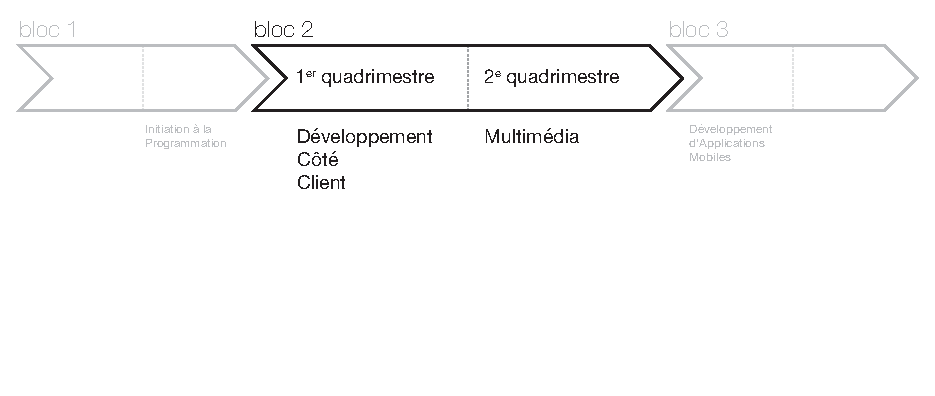
\includegraphics[width=\textwidth]{figures/corequis.eps}
        \caption{Illustration du corequis}
        \label{Fig:GQM}
    \end{center}
\end{figure}
\clearpage

\section{Contenus}

Voici dans l'ordre les différents thèmes que nous aborderons ensemble en classe. Les différentes séances de cours sont organisées avec une complexité croissante. Cela vous permet de mieux comprendre et de retenir les informations. Si le cours est trop complexe au début, vous pourriez vous sentir dépassés et perdre rapidement le fil de ce qui est enseigné. En organisant la complexité de manière progressive, vous avez le temps de comprendre les concepts de base avant de passer aux parties plus sophistiquées. Cela rend le cours plus agréable et engageant. Si le cours est trop difficile, vous pourriez perdre la motivation et l'intérêt.


\begin{enumerate}
    \item Test formatif en JavaScript.
    \item Correction et rappels des concepts de base JavaScript utilisés dans le cadre de ce cours.
    \item Utilisation d’un framework pour compiler les fichiers sources.
    \item Réalisation d'animations 2D simples avec JavaScript.
    \item Réalisation d’un outil qui permet de générer un logo à partir de paramètres encodé par l’utilisateur.
    \item Introduction à l’API de Canvas.
    \item Révision de quelques concepts mathématiques essentiels pour animer des formes. (Radian, degré, périmètres, Sin, Cos, etc.)
    \item Mise en place d’une boucle d’animation. Déplacer aléatoirement et à vitesse constante, des formes dans un canvas.
    \item Déplacer plusieurs formes avec la détection du survol de la souris.
    \item Détecter et interagir avec les évènements émis par l'utilisateur. Clic, survol, clavier, etc..
    \item Utilisez l’API Canvas pour appliquer des traitements sur des images bitmap.
    \item Déplacer des formes avec des images dans un canvas.
    \item Simuler de la neige, de la pluie sous l'effet du vent.
    \item Dessiner et animer le décor d’un jeu 2D avec une sprite sheet.
    \item Réalisation d’un premier jeu complet Flappybird.
    \item Réalisation d’un deuxième jeu complet Asteroids.
    \item Réalisation d’un examen formatif des années précédentes.
    \item Correction de l'examen formatif.
\end{enumerate}

\clearpage
\subsection{Justifications}

J'ai cherché à calibrer la complexité du cours pour permettre aux étudiants de mieux comprendre et de retenir les informations. Une étude menée par \citet{mayer2003nine} a montré que lorsque les étudiants apprennent de nouvelles informations de manière progressive, ils ont de meilleures performances que lorsqu'ils apprennent de manière non progressive. Cela s'explique par le fait que lorsque les étudiants apprennent de manière progressive, ils ont l'occasion de mettre en relation les nouvelles informations avec ce qu'ils savent déjà, ce qui peut les aider à mieux comprendre et retenir. \citet{gagne1974principles} rejoint cette idée. Si les étudiants sont constamment confrontés à des concepts difficiles, ils peuvent avoir du mal à suivre et à acquérir de nouvelles compétences de manière efficace. En organisant la complexité de manière progressive, les étudiants ont la possibilité de s'exercer et de mettre en pratique ce qu'ils ont appris avant de passer aux concepts plus difficiles.\\

Enfin, cela peut rendre le cours plus agréable et engageant pour les étudiants. Selon \citet{keller1987development}, la motivation des étudiants est influencée par leur perception de l'intérêt et de la pertinence du cours, ainsi que par leur perception de leurs propres compétences et de leur progression. Si le cours est trop difficile, les étudiants peuvent perdre la motivation et l'intérêt. En organisant la complexité de manière progressive, les étudiants peuvent sentir qu'ils progressent et atteignent des étapes importantes, ce qui peut renforcer leur engagement et leur motivation.

\clearpage
\section{Visées d’apprentissage}

Ce cours de «~multimédia~» vise à~:
\begin{enumerate}
    \item Développer votre aptitude à programmer en JavaScript. Plus exactement, à partir d'un énoncé, exprimé en français, proposer un programme en JavaScript \underline{efficace} dans \underline{un navigateur} qui respecte \underline{nos critères des qualités}. Ce qui implique de :
          \begin{enumerate}
              \item Connaitre les \underline{concepts} fondamentaux\footnote{Il s'agit là d'une dizaine de concepts qui reviennent tout le temps et qui seront identifiés en tant que tels.} utilisés dans la programmation avec JavaScript~;
              \item Comprendre ces concepts~;
              \item Identifier les concepts dont vous aurez besoin pour un cas pratique donné~;
              \item Savoir combiner différents concepts~;
              \item Savoir utiliser \underline{les outils de développement} vus en cours.\\
          \end{enumerate}
\end{enumerate}


Les mots ont de l'importance et je souhaite qu'on s'entende sur ceux-ci :

\begin{itemize}
    \item \underline{Concepts}~: c'est une «~idée~» ou une «~notion~» qui est importante et dont on a besoin pour programmer en JavaScript. Elle est utilisée pour comprendre et résumer quelque chose de manière générale~;
    \item \underline{Efficace}~: c'est à dire qui a été conçue de sorte à pouvoir fonctionner sans pour autant consommer \emph{inutilement} des ressources~;
    \item \underline{Nos critères des qualités}~: sont définies \href{https://github.com/tecg-dcc/dcc-guidelines}{ici}\footnote{github.com/tecg-dcc/dcc-guidelines} dans notre guide des bonnes pratiques. Ce sont ces règles que nous appliquons systématiquement en classes~;
    \item \underline{Un navigateur}~: je ne précise pas lequel, car vous devez utiliser les techniques vues en classe qui sont supportés par tous les navigateurs~;
    \item \underline{Les outils de développement}~: il s'agit là simplement des logiciels que nous utilisons en classes. Par exemple, PhpStorm, Git, Brave, etc.
\end{itemize}

\clearpage
\subsection{Justifications}

Je trouve cette partie particulièrement importante pour les étudiants. Finalement, c'est ici que je fixe mes attentes. J'ai donc essayé de les rendre aussi compréhensibles que possible à tel point que j'ai demandé à 2 de mes cousins, qui sont en 6\up{e} secondaire, de lire cette partie et de m’expliquer ce qu’ils comprennent. J'ai bien conscience du manque de rigueur et des lacunes que présente cette approche. L'intention étant ici, dans le temps qu'il m'est imparti, de tester la compréhension des visées. Bien entendu, il serait souhaitable de le faire avec \emph{mes} étudiants et un nombre plus important de sujets. Il n'empêche qu'à l’issue de cet échange, j'ai adapté l'écriture des visées d'apprentissage. Mes cousins avaient du mal avec certains mots. Je me suis donc permis de les définir pour que mes étudiants et moi ayons la même représentation derrière ces mots. Je n'ai pas mis en italique les verbes d'action de la taxonomie de Bloom afin d'éviter de distraire mes étudiants. Pour mes cousins, la mise en évidence de ces verbes ne les aidait pas à comprendre.\\

Ces précisions sur la \emph{forme} apportées, j'en viens au \emph{fond}. J'ai choisi de travailler avec une \emph{approche par objectifs (APO)}. Initialement, j’étais parti sur l’idée d’exprimer une seule compétence de très haut niveau, mais ce n'est pas ce qui correspond le mieux à la réalité. Je cherche à entrainer leur capacité à identifier les concepts dont ils ont besoin à partir d'une exigence formulée en français. Après avoir identifié ces concepts, ils doivent pouvoir les mettre en pratique. Ce sont toujours les mêmes concepts qui reviennent même si la combinaison peut être unique puisqu'elle dépend de l'exigence. Ils ne sont donc pas toujours dans des situations parfaitement nouvelles. Pour ce cours, je ne suis pas vraiment dans une approche par compétences, c’est plutôt une approche par objectifs. Je suis conscient des limites de cette approche. Par exemple, j'ai du mal à déterminer le niveau de spécificité. Par exemple, mes objectifs spécifiques pourraient encore être détaillés en donnant davantage de précision sur le contexte et sur la mesure de la performance, mais où placer le curseur ? Aussi les objectifs peuvent être artificiellement simples et par définition \emph{peu intégrés}. Je compense cela en essayant de formuler des objectifs de haut niveau qui justement ne se limite pas à la description d'une tâche simple, mais une tache intégrative et authentique. J'utilise la taxonomie de Bloom revue par \citet{anderson2001taxonomy} pour décrire mes objectifs. Pour deux raisons, elle est facile à comprendre pour mes étudiants et mes objectifs d'apprentissages sont du domaine cognitif.

Dans cette liste, je mets en relation les niveaux de la taxonomie de Bloom avec mes objectifs spécifiques. Comme on peut le voir, tous les niveaux sont exploités sauf l'\emph{'évaluation}, ce niveau qui vise à porter un jugement critique. Dans le cadre de ce cours, ce n'est pas ce que nous travaillons.
\begin{enumerate}
    \item \underline{Se rappeler} : Connaitre les concepts...
    \item \underline{Comprendre} : Comprendre les concepts...
    \item \underline{Appliquer} : Savoir utiliser les outils\footnote{Les outils sont les logiciels qu'ils utilisent pour programmer.} de développement...
    \item \underline{Analyser} : Identifier les concepts...
    \item \underline{Évaluer} :
    \item \underline{Créer} : Savoir combiner différents concepts... en vue de «~créer~»
\end{enumerate}

Au moment de rédiger ces lignes, ce cours est évalué de manière isolé. Mais il faut savoir qu'il s'agit là d'un des 3 langages fondamentaux du web. Nous (professeurs du bachelier) avons déjà évoqué plusieurs fois l'idée de proposer une seule tache intégrée avec ces deux autres cours. L'objectif serait alors de formuler des objectifs transversaux et de les évaluer de manière intégrée. À ce stade, nous sommes toujours en phase de réflexion, mais c'est vers cela que nous aimerions aller. Avec \emph{une approche programme}.

\clearpage
\section{Méthodes d’enseignement et activités d’apprentissage}

Vous avez choisi un bachelier professionnalisant, qui cherche donc à vous préparer, au mieux, au monde professionnel. C’est pourquoi j’ai choisi d’articuler le développement de vos compétences autour de cas réels issu de jeux vidéos. Ils permettent de comprendre concrètement et de manière interactive les concepts de la programmation dont vous avez besoin dans votre futur métier. Le cours se donne au deuxième quadrimestre, une fois par semaine à raison de 4~heures. Voici les types d'activités que vous allez vivre :
\begin{itemize}
    \item Je vous expliquerai de manière claire et concise, avec beaucoup d’exemples concrets, les concepts dont vous avez besoin pour programmer en JavaScript.
    \item Il y aura aussi des moments d'échanges, je vais vous faire réagir et débattre sur la matière que nous voyons. Je m'engage à organiser ces moments et à vous (re)focaliser sur la matière. Je m'engage aussi à mettre en lumière l'essentiel. En contrepartie, j’attends de vous que vous participiez en partageant vos idées et connaissances.
    \item Après avoir couvert un concept, vous allez réaliser des exercices en rapport avec celui-ci. On n’apprend pas seulement à rouler en lisant le Code de la route. Il faut s'entrainer. C'est pourquoi je vous apprends à combiner et manipuler les concepts que nous avons vus au travers d’exercices. Ces derniers couvrent progressivement la matière du cours. Ils vous entrainent de manière simple à la réalisation de tâches plus complexes, car même si un exercice peut paraitre facile l'idée qu'il y a derrière le concept restera vraie même pour les exercices plus récapitulatifs. Ces défis sont à réaliser en classe ou parfois en pleine autonomie chez vous. Ils feront l'objet d'une correction collective en classe. Dans tous les cas, toutes les solutions seront disponibles.
    \item À certains moments, vous allez devoir rechercher individuellement ou collectivement un concept à partir d'un problème que je vous pose.
    \item Création, à domicile et individuellement, durant les différentes semaines de cours, d'un exercice récapitulatif\footnote{Il s’agit là d’un jeu que vous aurez choisi (voir la section \ref{eval_formative} sur l’évaluation formative).}. Ici, il n'est plus question de s'entrainer sur quelques points de matière, mais d'en combiner beaucoup. Il s’agit là d’une occasion de vous entrainer à l’examen et de revoir les points de matière du cours. Je vous encourage, au fur et à mesure que nous voyons les concepts théoriques, de les mettre en pratique dans votre jeu.\\
\end{itemize}

Parmi nos outils de travail, j'apprécie particulièrement Moodle. Il nous rend bien des services. Je m'en sers pour publier, au fur et à mesure et avant chaque début de cours, la matière que nous allons voir ensemble. Cela permet de fournir une structure claire et logique qui vous aide à comprendre. Cela rend le cours plus engageant et agréable, car vous savez ce qui va se passer. Vous pourrez vous y préparer. Aussi cela peut vous servir si vous avez une absence. Ainsi vous pouvez, avec l'aide des autres étudiants, vous remettre en ordre. Bien entendu, j'y publie tous les supports de cours et ressources utilisés. Enfin, j’y mets en place un forum. Ce dernier vous permet de poser des questions sur les exercices qui vous posent problème en attendant le prochain cours. L'idée n'est pas de s'échanger la solution, mais de discuter de vos difficultés en vous aidant les uns les autres. Bien entendu, j'interviendrai toujours pour valider ou complémenter vos idées.\\

Cela fait maintenant plusieurs années que je mets en place ce mode de fonctionnement. Et je constate qu'il est encore plus efficace si vous avez une approche \emph{proactive}. Ce qui signifie prendre des initiatives et donc agir de manière anticipée plutôt que de simplement réagir aux évènements. Cela peut se manifester de différentes manières, par exemple en prenant l'initiative d'apprendre les concepts progressivement plutôt que d'attendre l'ultime moment. Être proactif peut être particulièrement utile pour vous, cela vous permet de prendre en main votre propre apprentissage et de mieux gérer votre temps et vos responsabilités.

\clearpage
\subsection{Justifications}

\citet{perrenoud1992differenciation} dit~: «~différencier, c’est organiser les interactions et les activités de sorte que chaque élève soit constamment ou du moins très souvent confronté aux situations didactiques les plus fécondes pour lui~». J’essaye donc, face à la diversité mathétique, d’apporter une polyvalence didactique. J'utilise la méthode des évènements d’apprentissage\cite{Leclercqevenements} pour varier mes méthodes d'enseignants~:
\begin{itemize}
    \item La transmission~: me permet de couvrir de façon structurée un grand nombre de concepts tout en contrôlant le rythme de l'apprentissage et de m'assurer que tous les étudiants suivent.
    \item Le débat~: il se présente de deux manières différentes. D'une part, pendant le cours (synchrone) quand je fais réagir les étudiants sur un concept. Mais aussi de manière asynchrone avec le forum. Puisqu'ils vont relire les propositions des autres pour y réagir et débattre. J'y interviens comme modérateur.
    \item L'exercisation : aussi simple que cela puisse paraitre, je pense que pour devenir un bon programmeur il faut programmer. Il faut s'entrainer et faire des exercices jusqu'à développer certains réflexes. C'est pourquoi les concepts théoriques que j'aborde avec eux n'ont de sens que s'ils les appliquent concrètement.
    \item L'exploration~: je le mets régulièrement en place pour introduire un nouveau concept. Je n'aime pas leur donner directement la solution. J'essaye de leur faire ressentir l'intérêt du concept au travers d'un problème. La solution à ce problème est le nouveau concept à découvrir. Dans un deuxième temps, je repasse sur de la transmission classique pour fixer le concept qu'ils ont exploré~;
    \item La création~: les étudiants ont un exercice récapitulatif à réaliser. Ce projet regroupe presque tous les concepts vus en classe. Pour ce projet, je guide mes étudiants. Je les aide en leur donnant du feedback individuel. J'en reparlerai dans la section \ref{eval_formative} sur l'évaluation formative.
    \item La métacognition~: quand je corrige les exercices avec les étudiants, je mets en lumière les stratégies qu'il faut mettre en place pour résoudre facilement l'exercice. Souvent, je demande, aux étudiants qui ont bien réussi l'exercice, d'expliquer aux autres comment ils ont procédé. J'espère ainsi leur donner une occasion de réfléchir à leur manière de penser et résoudre un exercice. Selon \citet{dunlosky2013improving},la métacognition peut aider les étudiants à réussir en leur permettant de planifier, surveiller et réguler leur propre processus de pensée et d'apprentissage.
\end{itemize}
\begin{figure}[H]
    \begin{center}
        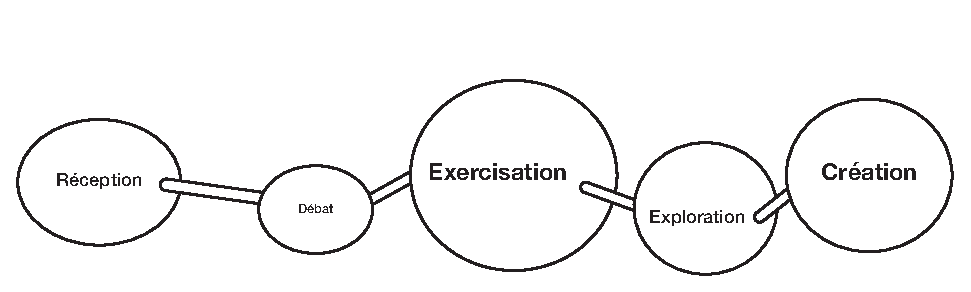
\includegraphics[width=0.9\textwidth]{figures/EAEs.eps}
        \caption{Représentation atomique de mes évènements dominants~\cite{leclercq2008modele}}
    \end{center}
\end{figure}
Le modèle de~\citet{perrenoud1992differenciation} me permet de décrire de manière précise mes méthodes d'enseignement. Ce qui est très intéressant d'observer, c'est que je ne couvre pas tous les évènements. Par exemple, je pourrais davantage voir comment mettre en place de l'expérimentation et ce que cela apporterait aux étudiants. Par exemple, je pourrais leur fournir des programmes partiels et eux devraient essayer de les compléter avec un nouveau concept, ce serait une forme d’exploration. Je pense aussi que l'imitation pourrait avoir une place plus importante. Cela intervient de manière ponctuelle quand je leur montre comment je configure certains outils, mais ce n'est pas assez représentatif que pour en parler ici.

J'aimerais apporter une précision sur \emph{l’exercisation} qui occupe une part importante du cours. De prime à bord on pourrait se dire que cet évènement pourrait être ennuyeux et manquer de sens pour les étudiants s'ils ne comprennent pas pourquoi ils sont censés le faire. C'est pour cela que je recontextualise systématiquement l'exercice. Je veux que mes étudiants sachent pourquoi la réalisation est pertinente pour leur apprentissage. De plus, si l'exercice est trop difficile ou trop facile, il peut décourager et nuire à leur motivation. C'est pour cela que je les entraine \emph{concept par concept}. Je les ajoute progressivement tout en essayant d'avoir un bon équilibre de sorte à les stimuler sans pour autant les décourager par la complexité. Aussi quand un étudiant termine un exercice, avant les autres, je lui propose une variation de l'exercice un peu plus compliqué. Je ne voudrais pas que les meilleurs étudiants s'ennuient à attendre les autres.\\

Comme on peut le lire dans la partie pour les étudiants, je les rassure sur l'idée que derrière les exercices d'apparence simple se cachent des invariants qu'ils doivent réappliquer pour les exercices plus intégratifs. D'ailleurs, \citet{piaget1970structures} en parle dans ses travaux sur le développement cognitif de l'enfant. Selon lui les \emph{invariants opératoires} sont des structures mentales qui permettent à l'enfant de traiter l'information de manière cohérente et de résoudre des problèmes \cite{piaget1970structures}.

Il identifie deux types d'invariants opératoires : les \emph{invariants formels} et les \emph{invariants opérationnels concrets}. Les invariants formels sont des structures mentales abstraites qui permettent à l'enfant de traiter des informations symboliques, comme les nombres ou les lettres. Les invariants opérationnels concrets sont des structures mentales qui permettent à l'enfant de traiter des informations concrètes, comme les objets ou les actions.

Tourjours selon \citet{piaget1970structures}, l'acquisition des invariants opératoires est un processus progressif qui se déroule en plusieurs étapes. L'enfant commence par acquérir des invariants opérationnels concrets, puis il passe aux invariants formels. Cette progression permet à l'enfant de développer de plus en plus de capacités de raisonnement et de logique.

Dans mon cours ces invariants opératoires sont utilisés pour les  aider à comprendre les concepts abstraits puis à résoudre les tâches plus complètes.\\

«~Make learning visible~» \footnote{«~The 'visible' aspect also refers to making teaching visible to the student, such that they learn to become their own teachers.~»\cite{hattie2012visible}}\cite{hattie2012visible}. Le projet est aussi une occasion, pour les apprenants (et moi-même), de se rendre compte des savoirs qu'ils acquièrent. Ils voient bien qu'au fur et à mesure que la matière est vue, ils peuvent avancer dans la réalisation de leur propre jeu.\\
Étant donné que la motivation fait partie de ma philosophie et que l’un des ingrédients de la motivation c’est d’apporter de la valeur aux connaissances\cite{viau1994motivation}, ce projet me permet de rendre concrets mes enseignements au travers de besoins issus de situations authentiques.\\

J'accorde une grande importance à la correction des exercices. Cela me semble encore plus important que l'exercice isolément. En début de séance, je demande aux apprenants s'ils souhaitent que je corrige, avec eux, un exercice qui leur semble particulièrement difficile. S’ils n’ont pas de souhaits particuliers, je corrige quand même au moins un exercice pour vérifier la compréhension. C'est une occasion pour eux d’avoir du feedback. J'y accorde beaucoup d'importance, car selon selon \citet{hattie2007power}, le feedback peut aider les étudiants à comprendre ce qu'ils ont bien fait et ce qui peut être amélioré, ce qui peut les motiver à continuer à apprendre et à progresser. C'est aussi une occasion pour moi de leur communiquer de manière concrète mes critères de qualité et les normes de performance attendues. Ce qui, selon \citet{sadler1989formative}, peut les aider à se fixer des objectifs d'apprentissage plus élevés. \\

\clearpage
\section{Évaluation des apprentissages}

\subsection{L’évaluation formative}
\label{eval_formative}

Ces 2~évaluations formatives ont pour but de vous entrainer. De vous offrir une situation authentique supplémentaire pour vous exercer sans pour autant vous pénaliser. Ce qui m'importe ici, c'est que vous appreniez.
\begin{enumerate}
    \item Lors de la première séance~: vous réaliserez un test formatif d’application pratique sur la matière du cours de «~Développement Côté Client~» qui est le corequis de ce cours. Ceci est une occasion pour vous et moi de mesurer votre maitrise en JavaScript.
    \item Lors de l'avant-dernière séance de cours~: vous réaliserez individuellement un examen des années précédentes en classe. Nous consacrerons la dernière séance à sa correction collective où chacun corrige individuellement sa copie d'examen.
\end{enumerate}

\subsection{L’évaluation certificative}
\subsubsection{Première session}
\label{eval_certificative}
L’évaluation certificative s'organise en 2~temps~:
\begin{enumerate}
    \item Vous devez rendre, le jour de l'examen, votre projet de jeu personnel que vous aurez développé individuellement chez vous pendant les différentes semaines de cours. Les consignes vous seront communiquées au premier cours. Vous devez donc gérer votre temps pour ce projet qui compte pour 20~\% de la cote finale.
    \item L'examen pratique consiste à programmer un jeu à partir d'un énoncé\footnote{Je vous rappelle que les énoncés des années précédentes sont disponibles sur l'\href{https://github.com/tecg-mmi}{organisation GitHub} officielle du cours. (github.com/tecg-mmi)} qui vous sera fourni et que vous découvrirez le jour même. Vous aurez à votre disposition toutes les ressources du cours, un accès complet aux documentations officielles, ainsi que vos propres productions. Vous disposez de 4~heures pour réaliser cet examen en classe. Ce travail compte pour 80~\% de la cote finale.
\end{enumerate}
Lors de la première séance de cours, je vous présenterai l'énoncé du dernier examen avec sa grille d'évaluation. Elle se construit toujours de la même manière. J'attribue aux fonctionnalités du jeu un degré de complexité. Ensuite, je mesure l'aboutissement des différentes fonctionnalités dans votre proposition. Ces fonctionnalités sont clairement mentionnées dans l'énoncé de l'examen et sont classées par ordre de complexité. Le nombre de points maximum attribué à chaque fonctionnalité est également mentionné.

J'ai pour objectif de vous mettre, le plus possible, dans des situations de travail réalistes. C'est-à-dire celles que vous pourriez possiblement rencontrer dans un futur métier et même votre premier emploi. C'est donc pour cela que l'examen se fait sur vos machines à cours ouvert avec la documentation officielle ainsi que vos productions personnelles. Notez cependant que la limite à ne pas franchir c'est la communication avec autrui\footnote{"Autrui" désigne une personne ou un groupe de personnes différentes de soi-même.}. D'ailleurs, vous passerez l'examen au Léo sous ma surveillance.
\subsubsection{Deuxième session}


\subsection{Justifications}
\label{evaluation_des_apprentissages_justifications}
\begin{itemize}
    \item Parler l'authentissité…
    \item Parler de la motivation intrinsèque. On ne travaille pas que pour des points. On travaille aussi pour soi.\todo{text}
    \item «~L’émission de feedbacks est souvent considérée comme un élément clé pour renforcer la motivation et soutenir la réussite des élèves.~»\cite{georges2011feedbacks}. La réalisation de l'examen formatif est une activité intégrée qui permet de recevoir du feedback. D'une part, sur sa compréhension de la matière, donc plutôt un feedback simple de type assertif et évaluatif\cite{georges2011feedbacks} sur sa performance. D'autre part un feedback plus complexe relatif aux stratégies qu'il faut adaptées (Métacognition). Par exemple, quelles sont les parties plutôt simples et comment rapidement les valider. Ou encore, réfléchir aux éléments plus compliqués, que mes apprenants aiment appeler des «~pièges~»\footnote{Je n'adhère évidemment pas à cette appellation. Mon examen ne contient pas de «~pièges~» sans quoi on pourrait se poser des questions sur mes intentions. L'examen contient des parties plus compliquées qui nécessitent une certaine forme d'inhibition cognitive.}. \citet{hattie2008visible} explique dans son ouvrage que le feedback a un impact significatif sur la performance de l'apprenant. Enfin, c'est une occasion pour entrainer la méta-cognission\cite{leclercq2008modele}. Nous réfléchissons ensemble aux stratégies qu'il faut mettre en place pour réussir l'examen. D'ailleurs chaque année je désigne un «~sécrétaire~» pour cette séance. Il aura pour mission de prendre note de toutes les astuces que nous avons déterminées ensemble afin que les apprenants puissent consulter cette ressource plus tard. D'autre part, je prends soin, dans la rédaction de l'énoncé, d'être constant. À vrai dire, je réutilise un template de base pour rédiger l'énoncé d’examen afin qu’ils ne soient pas surpris par la forme le jour de l'examen.
    \item La réalisation de l'exercice formatif est l'occasion pour moi de me rendre compte des éventuelles lacunes de certains apprenants. Cela me donne une vision assez précise de leur niveau. Je peux donc donner un feedback personnalisé et leur fournir des ressources spécifiques au besoin.
    \item Je choisis de présenter lors de la \textit{first-class meeting}, après la fiche ECTS, la grille d'évaluation afin de permettre à tout le monde d'éventuellement adapter des stratégies de réussite et aussi pour rendre très concrète la compétence visée. Ainsi ils savent, dès le début, où se trouvent la fiche et les examens des années précédentes.
\end{itemize}

\section{Alignement pédagogique}
\begin{table}[H]
    \begin{tabular}{|l|l|}
        \hline
        Visées d’apprentissage        & \begin{tabular}[c]{@{}l@{}}Savoir programmer dans un navigateur avec l'API de canvas un jeu.\end{tabular}                                                                                                                                                                                                                                                           \\ \hline
        Activités d’apprentissage     & \begin{tabular}[c]{@{}l@{}}–~Exercice pratique par matière\\ –~Entrainement à l’examen\\ –~Exploitation collective ou individuelle de nouvelles \\  techniques pour proposer des solutions.\\ –~Apprentissage par projets avec le projet personnel.\\ –~Transmission théorique.\end{tabular}                                                                        \\ \hline
        Évaluation des apprentissages & \begin{tabular}[c]{@{}l@{}}\\1. Création, à domicile et individuellement, durant les différentes\\semaines de cours, d'un jeu personnel à 2~dimensions,\\dans un navigateur avec l'API de canvas. \\2. Création lors de la session d'examens en classe\\et individuellement, d'un jeu imposé à 2~dimensions,\\dans un navigateur avec l'API de canvas.\end{tabular} \\ \hline
    \end{tabular}
\end{table}
%% Attention.... il faut dire... Vous voyer pourquoi on a été fait ça ? C'est pour que vous soyez capable de faire ceci... 

\subsection{Justifications}
\begin{itemize}
    \item La compétence que je souhaite entrainer, c'est la programmation d'interfaces multimédias riches dans un navigateur, en me limitant aux jeux 2D.
    \item Je les y entraine au travers de différentes activités d'apprentissages variées afin de répondre à la différence mathétique des apprenants. Dans tous les cas, toutes ces activités visent un même objectif. Construire ensemble les briques nécessaires à la réalisation d'un jeu en pleine autonomie.
    \item Enfin, j'évalue, à la fin, la capacité de l'apprenant à réaliser, en pleine autonomie, un jeu à 2~dimensions dans un navigateur avec l'API de canvas.
\end{itemize}
\clearpage

\section{Modalités organisationnelles}
\subsection{Comment me contacter}
\begin{enumerate}
    \item Pour toutes les communications d'ordre personnel, je vous demande de me contacter par mail \href{mailto:daniel.schreurs@hepl.be}{daniel.schreurs@hepl.be}.
    \item Si vous avez des questions techniques liées à une incompréhension et/ou un problème avec un exercice, je vous demanderai de la poser sur le forum officiel du cours sur Moodle. Cela permettra de faire profiter tout le monde de votre question.
    \item Si vous avez des informations urgentes à me faire parvenir, vous pouvez me joindre directement via Teams que j'ai installé sur mon téléphone.
\end{enumerate}
\section{Ressources}
\begin{itemize}
    \item Moodle~: toutes les ressources nécessaires pour le cours sont référencées sur la page officielle du cours. Je choisis cette plateforme, car c'est l'outil officiel recommandé et utilisé au sein de la HEPL. Vous y trouverez des sections avec~:
          \begin{itemize}
              \item Le déroulement de toutes les séances de cours~: avec la matière couverte et les liens vers les ressources utilisées lors de cette séance. Ainsi vous avez une trace écrite de ce que nous avons vu à chaque séance.
              \item La fiche ECTS~: présenté au premier cours pour que vous poussiez la relire.
              \item Le forum~: qui vous permet de poser des questions tout en faisant profiter tout le monde.
              \item Les notes de cours au format PDF et Microsoft PowerPoint\footnote{Je vous donne également ce format, car je sais que certains étudiants aiment prendre note dans la partie "note de l'intervenant".}, ainsi vous pouvez les télécharger avant le cours et les annoter pendant que je donne les explications.
              \item Toutes les ressources auxiliaires~: que j'utilise en classe.
          \end{itemize}
    \item Logiciels nécessaires~: Il est indispensable d'avoir un environnement de travail informatique opérationnel. Nous utiliserons la même configuration de machine que pour le cours de «~Développement Côté Client~». Vous pouvez retrouver toutes les installations à faire \href{https://github.com/tecg-dcc/js-ressources#environnement-de-travail}{ici}\footnote{github.com/tecg-dcc/js-ressources}.
\end{itemize}
\clearpage
\section*{Réflexion personnelle}

Quand on m'a présenté les fiches ECT à la HEPL, je n'avais pas ressenti l'intérêt pour mes étudiants. Je pensais qu'il s'agissait d'une formalité admistrative. À l'issue de cette rédaction, je suis maintenant convaincu qu'ils  servent à motiver mes étudiants et à communiquer avec eux de manière clair et transparente. Cette rédaction a aussi été pour moi une occasion de réfléchir sur ce que je fais et pourquoi je la fais. Même si, bien sûr, je cherche toujours à assurer un alignement pédagogique, je me rends compte qu'il y moyen d'améliorer cela. Ce travail m'a aussi fais réagir sur la manière dont je me communique avec mes étudiants. Je me souviens, quand j'étais petit, je ne supportais pas qu'on impose quelque chose de manière péremptoire, sans une explication valable. Je me suis souvenu de ça tout du long de cette rédaction. J'ai particulièrement soigné la justification à l'égard de mes étudiants. J'ai esssayé tant que possible de toujours expliquer pourquoi je fais les choses et pourquoi de cette manière là. Cela peut paraitre assez trivial quand c'est présenter ainsi mais dans les faits je trouve que je manque un peu de temps au début de mon parcours. Et donc il m'arrive parfois d'oublier de rappaler le pourquoi du comment.
\\
Ce travail a été pour moi une occasion de lire beaucoup de litérature. C'est sans doute ce qui explique pourquoi cela m'a pris autant de temps. Quand je parle d'une mes partique j'ai maintenant pris l'habitude de voir si d'autres n'ont pas déjà investiguer cette manière de faire. Bien souvent la réponse est oui. Et donc j'ai pû grace à ce travail comparer mes pratiques d'enseignants en vue de les améliorer. Nous avons la chance d'avoir accès à temps de ressources et donc d'expériences autant les mettre à projet de mettre à profil l'expérence de nos pères.

\clearpage
\section{Bibliographie}
\printbibliography[heading=none]

%\bibliography{citations}
%\bibliographystyle{apalike-fr}





\end{document}
